%%%%%%%%%%%%%%%%%%%%%%%
%                                                   %
%                 Experiment H-01                   %
%         Experiment Title  Ideal Gas Law           %
%                                                   %
%%%%%%%%%%%%%%%%%%%%%%%

%\labChapter{H}{[1145L] - Ideal Gas Law}
\labChapter{H}{[1145L - LIFE SCIENCES / algebra-based course] --- Ideal gas law with Isothermal \& Adiabatic Compression;  Estimating Absolute Zero}
\label{lab:H7_1145L}

\section{Background}

A general and complete description of an ensemble of many atoms or molecules is a very difficult, if not impossible task, given the large number of objects involved. Luckily enough most gases follow a relatively simple approximation for a rather large range of conditions.

The ideal gas law describes the behavior of a gas of point-like
particles.  While there is no such thing as an ideal gas (all real
molecules have a small but non-zero size), it is nevertheless a good
approximation to the behaviour of gasses at ordinary temperatures and
pressures.

\subsection{Ideal Gas Law}

The Ideal Gas Law assumes that
\begin{itemize}
\item[$\triangleright$] The gas is made up of molecules moving in straight lines, but random directions,
  %\item[$\triangleright$] The molecules in the gas behave as if they were rigid spheres,
\item[$\triangleright$] All collisions between the molecules themselves and between the molecules and the walls of the container are perfectly elastic,
\item[$\triangleright$] The temperature of the gas is directly proportional to the kinetic energy of the molecules,
\item[$\triangleright$] The pressure of the gas is due to the collisions of the molecules with the walls of the container,
\item[$\triangleright$] All inter-molecular forces can be neglected, and
\item[$\triangleright$] The volume occupied by the molecules is negligible as compared to the volume of the container.
\end{itemize}
Under these conditions the pressure, temperature, and volume of the gas will follow a simple relationship,
\begin{equation}
  \label{eq:idealgas}
  P V = n R T
\end{equation}
where
$P$ is the gas pressure in Pascals ($1\,\pascal = 1\,\newton\per\metre\squared$), $T$ is the gas temperature in Kelvin, $V$ is the volume (in \metre\cubed), and $n$ is the number of moles in the gas ($1\,\mole = 6.022\times10^{23}\,\mbox{molecules}$).  $R$ is called the universal gas constant and for these units has the value $R = 8.3145\,\joule\per\mole\per\kelvin$.

Most gases will behave approximately as an ideal gas within a certain range of conditions, but the law fails at low temperatures or higher pressures when forces between the gas molecules become important.

\subsection{Absolute Zero}

One of the things the ideal gas law assumes is that the kinetic energy of the gas molecules is directly proportional to the temperature of the gas. Therefore, if the molecules have no kinetic energy (the molecules are at rest) then the temperature of the gas is at its lowest possible value. This temperature is called absolute zero and is used as the zero-point of the Kelvin temperature scale
\[
0\,\kelvin = -273.15\,\celsius.
\]
Note that, according to the definition of pressure, gas molecules at absolute zero will also exert no pressure on the walls of the container the gas is in.

\section{Experimental Procedure}

This experiment uses temperature and pressure sensors plugged into an interface so that data for both variables can be recorded simultaneously.
For the Ideal Gas Law experiment the air inside a syringe is compressed by pushing on the plunger. Pressure and temperature values are collected and recorded with the Capstone program, which is then also used to analyze the data. See page~\ref{sec:SettingUpHardware} for guidance.
For the Absolute Zero experiment a hollow sphere (with a fixed volume) is submerged in liquids of different temperature. Capstone will again collect and record pressure and temperature data of the gas enclosed in the sphere.
Pictures of the experimental setups are shown in Figures~\ref{H01Fig01} and \ref{H01Fig02}.

\begin{figure}
  \begin{center}
    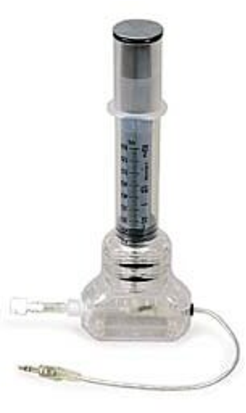
\includegraphics[width=1.5in]{Experiment10Figures/Figure01a.pdf}\hspace{2cm}
    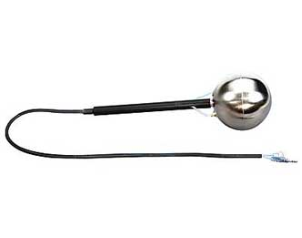
\includegraphics[width=2.0in]{Experiment10Figures/Figure01b.pdf}
  \end{center}
  \caption{The left picture shows the Ideal Gas Law experiment without the PasPort interface. The two cables coming from the syringe are the temperature and pressure connectors. The plunger of the syringe has a mechanical stop to prevent full compression of the syringe.
    The right-hand picture shows the Absolute Zero experiment, again without the PasPort interface. The pressure and temperature connectors are shown exiting at the end of the black cable of the device.}
  \label{H01Fig01}  % the \label command comes AFTER the caption
\end{figure}

\begin{figure}
  \begin{center}
    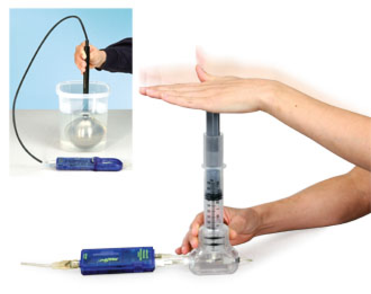
\includegraphics[width=4.0in]{Experiment10Figures/Figure02.pdf}
  \end{center}
  \caption{This picture shows the experimental methods for the Ideal Gas Law (main picture) and Absolute Zero (inlet) experiments. In both cases the temperature and pressure connectors are plugged into the PasPort interface (the small blue box).}
  \label{H01Fig02}
\end{figure}

% Ideal Gas Law
\subsection{The Ideal Gas Law Experiment}

\begin{itemize}
\item[$\triangleright$] Create a Part~1 Data Table for your ideal gas law measurements and calculations. 
\item[$\triangleright$] Open graphs of absolute pressure ($y$-axis) vs. time ($x$-axis) and temperature in Kelvin ($y$-axis) vs. time ($x$-axis) in the \textbf{Capstone} program. Also have a table displaying absolute pressure and temperature open. All these can be opened by double-clicking on the corresponding items on the right-had side of the \textbf{Capstone} program.
\item[$\triangleright$] Disconnect the quick-release pressure connector and push the plunger all the way down. Note that the mechanical stop will prevent the plunger from being pushed all the way to the bottom of the syringe. Record the volume reading on the syringe as the volume $V_{2}$ in your Part~1 Data Table. The value for $V_{2}$ should be about 20 cc.
\item[$\triangleright$] Set the plunger for an initial volume of $V_{1} = 40\,\centi\meter\cubed$.
\item[$\triangleright$] After you have adjusted the volume, re-connect the pressure port.
\item[$\triangleright$] Hold the base of the syringe firmly against a sturdy, flat surface (the lab table).
\item[$\triangleright$] Press the \textbf{Record} button on \textbf{Capstone}.
\item[$\triangleright$] Press straight down as hard as you can on the plunger with the palm of your hand to fully compress the gas inside the syringe. Keep pressing to hold the pressure steady. Important: Do not let the pressure drop for at least 30 s. The mechanical stop will prevent you from decreasing the volume of the gas to less than than about 20 cc. Hold this position until the temperature and pressure have stabilized and are no longer changing (use the data table as an indicator). It should take less than 30 seconds for the temperature to return to room temperature.
\item[$\triangleright$] Release the plunger and allow it to expand back out on its own (it may not go back to 40 \centi\meter\cubed). Wait again until the temperature and pressure have equalized and are no longer changing.
\item[$\triangleright$] Press the \textbf{Record} button again on \textbf{Capstone} to stop recording data.
\end{itemize}


% Analysis with Constant Temperature
\subsubsection{Analysis with Constant Temperature}
\begin{itemize}
\item[$\triangleright$] Highlight an area (click and drag with the mouse) on the pressure graph at the beginning of the data-collecting run, before you compressed the air in the syringe. The highlighted values of the selected data points will appear in the data table of \textbf{Captone}. Record the initial pressure as $P_{1}$ in your Part~1 Data Table.
\item[$\triangleright$] Highlight an area on the pressure graph at the point just before you released the plunger. Record the final pressure as $P_{2}$ in your Part~1 Data Table.
\item[$\triangleright$] Calculate the ratio of initial volume over the final volume, $X_{1} = \nicefrac{V_{1}}{V_{2}}$ and record the result in your Part~1 Data Table.
\item[$\triangleright$] Calculate the ratio of final pressure over the initial pressure, $X_{2} = \nicefrac{P_{2}}{P_{1}}$ and record the result in your Part~1 Data Table.
\item[$\triangleright$] Compare the two ratios. According to the ideal gas law (Eqn.~\ref{eq:idealgas}) the two values should be equal, since $P_{1} V_{1} = P_{2} V_{2}$ for constant temperature (note that the temperature is room temperature in both cases). Discuss, first amongst yourselves and then with your instructor, why the values are different.
\end{itemize}

% Analysis with Varying Temperature
\subsubsection{Analysis with Varying Temperature}

By now you have (hopefully) figured out that you have not accounted for the small amount of volume of air inside the tubing of the apparatus. Using the ideal gas law (Eqn.~\ref{eq:idealgas}) and the data you collected in part 1 you can actually calculate this volume $V_{0}$ by solving the following equation for $V_{0}$
\begin{equation}
  \frac{(V_{1} + V_{0})}{(V_{2} + V_{0})} = \frac{P_{2}}{P_{1}}.
\end{equation}

Using the data from your Part~1 Data Table calculate the value for $V_{0}$ and note the result in your Part~2 Data Table.
\begin{itemize}
\item[$\triangleright$] Highlight an area (click and drag with the mouse) on the temperature graph at the beginning of the data-collecting run, before you compressed the air in the syringe. The highlighted values of the selected data points will appear in the data table of \textbf{Capstone}. Record the initial pressure and the initial temperature as $P_{1}$ and $T_{1}$ in your Part~2 Data Table.
\item[$\triangleright$] Note the initial volume $V_{1}^\prime = V_{1} + V_{0}$ in  your Part~2 Data Table.
\item[$\triangleright$] Highlight the area (click and drag with the mouse) on the temperature graph where the temperature peaks. The highlighted values of the selected data points will appear in the data table of \textbf{Capstone}. Note the peak temperature and the corresponding pressure at this instant as $P_{2}$ and $T_{2}$ in  your Part~2 Data Table.
\item[$\triangleright$] Note the volume $V_{2}^\prime = V_{2} + V_{0}$ in your Part~2 Data Table.
\item[$\triangleright$] Calculate the ratio $Y_{1} = \nicefrac{P_{1} V_{1}^\prime}{T_{1}}$ and record the result in your Part~2 Data Table.
\item[$\triangleright$] Calculate the ratio $Y_{2} = \nicefrac{P_{2} V_{2}^\prime}{T_{2}}$ and record the result in your Part~2 Data Table.
\item[$\triangleright$] Assuming the most significant error is in the volume, compare the difference between the two ratios with your estimate of the uncertainty in the volume.
\end{itemize}

% Measurement of Absolute Zero
\subsection{Measurement of Absolute Zero}

\begin{itemize}
\item[$\triangleright$] Connect the Absolute Zero apparatus to the PasPort system (both the temperature sensor and the quick-release pressure port need to be connected).
\item[$\triangleright$] Close the \textbf{Capstone} Program and re-open it from the desktop.
\item[$\triangleright$] Open a {\bf Table \& Graph} from the main canvas of \textbf{Capstone}. For the $x$-axis of the graph select absolute pressure and for the $y$-axis select temperature in \celsius. For the data table select the same two variables.
\item[$\triangleright$] Now click on the \textbf{Continuous Mode} and select \textbf{Keep mode} from the pull-down menu that will appear. Click on the \textbf{Preview} button to start collecting data.
\item[$\triangleright$] Run the hot water until steam rises from the sink. Fill a pitcher to the 2 quart mark. 
\item[$\triangleright$] First fully submerge the sphere in hot water: Observe the data points appearing on the graph. Make sure the sphere stays completely submerged the entire time you take data. Once the temperature has reached equilibrium (i.e.\ the value in the digital display no longer changes), press the \textbf{Keep Sample} button (N.B.\ Do \textbf{NOT} stop the data collection by clicking on the red square button again). Read and note the values for pressure and temperature (from the digital display) in  your Part~3 Data Table.
\item[$\triangleright$] Next remove half of the water in your container and replace it with cold water from the sink. Again fully submerge the sphere in the water and make sure the sphere stays completely submerged the entire time you take data. Note how the point moves in the Temperature vs. Pressure graph as the values change. Discuss the outcome among yourselves and with your instructor. Once the temperature is stable again (this will take a few minutes) press the \textbf{Keep Sample} button again. Read off and note the values for pressure and temperature (from the digital display) in your Part~3 Data Table.
\item[$\triangleright$] Lastl submerge the sphere in the cold water. Once again you need to make sure the sphere is completely submerged during the time you take data. Note how the point moves in the Temperature vs. Pressure graph as the values change. Discuss the outcome among yourselves and with your instructor. Once the temperature is stable again (this will take a few minutes) press the \textbf{Keep Sample} button again. Read off and note the values for pressure and temperature in your Part~3 Data Table.
\item[$\triangleright$] Press the \textbf{Record}  button once again on DataStudio to stop recording data.
\item[$\triangleright$] Using the fitting tool in \textbf{Capstone}, fit a straight line to the 3 data points you have taken.
\item[$\triangleright$] The $y$-intercept of the best-fit line is the value for absolute zero temperature. Discuss among yourselves and with your instructor why this is the case. Note the result as $T_{0}$ in your Part~2 Data Table.
\item[$\triangleright$] Compare your result to the accepted value of $-273.15\,\celsius$.
\end{itemize}

\section{Data Analysis}

\begin{itemize}
\item[$\triangleright$] Create a table for the analysis at constant temperature including the measured values $V_1, P_1, V_2, P_2$ and the calculated values  $X_1, X_2$.
\item[$\triangleright$] Create a table for the analysis with varying temperature including $V_0, V_1, P_1, V_2, P_2$ and the calculated values  $V^\prime_1, V^\prime_2, Y_1, Y_2$.
\item[$\triangleright$] Create a table for the measurement of absolute zero including the pressure and temperature you measured at the hot, warm and cool temperatures as well as the $y$-intercept and the accepted value of $-273.15\,\celsius$.
\end{itemize}


See Interpretation of Results on next page $===>$

\pagebreak

\section{Post-Lab Submission --- Interpretation of Results}
\begin{itemize}
    \item Make sure to submit your finalized data table (Excel sheet)
    \item Constant Temperature (Isothermal):
        \begin{itemize}
            \item What properties of a system must be proportional if compression is isothermal?
            \item How do the two ratios, $X_{1}$ and $X_{2}$, compare?
            \item What may cause a discrepancy between the ratios of volumes and pressures?
        \end{itemize}
    \item Varying Temperature (Adiabatic):
        \begin{itemize}
            \item What properties of a system must be proportional if compression is adiabatic?
            \item How do the two ratios, $Y_{1}$ and $Y_{2}$, compare?
            \item What may cause a discrepancy between the ratios of volumes and pressures?
            \item Consider the uncertainty as due to volume, do the ratios agree based on that uncertainty range?
        \end{itemize}
    \item Absolute Zero:
        \begin{itemize}
            \item What does absolute zero represent about a system?
            \item What is your extrapolated result for absolute zero; how does it compare to the accepted value?
            \item What measurement uncertainties exist; how do they affect your determined value for absolute zero?
        \end{itemize}
    \item What are possible systematic errors for today's experiments?
\end{itemize}